
%\documentclass[spanish,a4paper,12pt,oneside]{extreport}
\documentclass[a4paper,12pt,oneside]{report}

% Fonts
% For use with XeLaTeX
\usepackage{amsmath}
\usepackage{fontspec}
\setmainfont[%
  Path              = ./fonts/ArgentumSans/,%
  Extension         = .ttf,
  UprightFont       = *-Light,
  BoldFont          = *-SemiBold, % ULL bold font
  ItalicFont        = *-LightItalic,
  BoldItalicFont    = *-SemiBoldItalic, % Linux Libertine O Regular Semibold Italic
  Scale             = 0.95%
]%
{hinted-ArgentumSans}

\usepackage{graphicx}
\usepackage[utf8]{inputenc}
\usepackage[spanish]{babel}

%\usepackage{alltt}

%\usepackage[ruled,vlined,commentsnumbered,linesnumbered,inoutnumbered,titlenotnumbered,noend]{algorithm2e}
%\SetKwRepeat{Do}{do}{while}
%
%\usepackage{multirow}
%\usepackage{array} 
%\usepackage{amsfonts}
%\usepackage{amsmath}
%\usepackage{bigstrut}
%\usepackage{booktabs}
%\usepackage{caption}
%\usepackage{chngpage}
%\usepackage{float}
%\usepackage{enumitem,lipsum}
%\usepackage{graphicx}
%\usepackage{lscape}
%\usepackage{microtype}
%\usepackage{natbib}
%\usepackage{pdflscape}
%\usepackage{rotating}
%\usepackage{subcaption}
%\usepackage{ctable}
\usepackage{hyperref}
%\usepackage{enumerate}
%\usepackage{gensymb}
%\usepackage{eurosym}
%\usepackage{xcolor}
\usepackage{tabu}
%
%\usepackage{lineno}
%%\\linenumbers
%\setlength\linenumbersep{5pt}
%\renewcommand\linenumberfont{\normalfont\tiny\sffamily\color{gray}}

\usepackage[top=2cm, bottom=2cm, left=2cm, right=2cm]{geometry}

\newenvironment{sourcecode}
{\begin{list}{}{\setlength{\leftmargin}{1em}}\item\scriptsize\bfseries}
{\end{list}}

\newenvironment{littlesourcecode}
{\begin{list}{}{\setlength{\leftmargin}{1em}}\item\tiny\bfseries}
{\end{list}}

\newenvironment{summary}
{\par\noindent\begin{center}\textbf{Abstract}\end{center}\begin{itshape}\par\noindent}
{\end{itshape}}

\newenvironment{keywords}
{\begin{list}{}{\setlength{\leftmargin}{1em}}\item[\hskip\labelsep \bfseries Keywords:]}
{\end{list}}

\newenvironment{palabrasClave}
{\begin{list}{}{\setlength{\leftmargin}{1em}}\item[\hskip\labelsep \bfseries Palabras clave:]}
{\end{list}}

\usepackage{listings}
\usepackage{xcolor}

\colorlet{punct}{red!60!black}
\definecolor{background}{HTML}{EEEEEE}
\definecolor{delim}{RGB}{20,105,176}
\colorlet{numb}{magenta!60!black}

\lstdefinelanguage{json}{
    basicstyle=\normalfont\ttfamily,
    numbers=left,
    numberstyle=\scriptsize,
    stepnumber=1,
    numbersep=8pt,
    showstringspaces=false,
    breaklines=true,
    frame=lines,
    backgroundcolor=\color{background},
    literate=
     *{0}{{{\color{numb}0}}}{1}
      {1}{{{\color{numb}1}}}{1}
      {2}{{{\color{numb}2}}}{1}
      {3}{{{\color{numb}3}}}{1}
      {4}{{{\color{numb}4}}}{1}
      {5}{{{\color{numb}5}}}{1}
      {6}{{{\color{numb}6}}}{1}
      {7}{{{\color{numb}7}}}{1}
      {8}{{{\color{numb}8}}}{1}
      {9}{{{\color{numb}9}}}{1}
      {:}{{{\color{punct}{:}}}}{1}
      {,}{{{\color{punct}{,}}}}{1}
      {\{}{{{\color{delim}{\{}}}}{1}
      {\}}{{{\color{delim}{\}}}}}{1}
      {[}{{{\color{delim}{[}}}}{1}
      {]}{{{\color{delim}{]}}}}{1},
}

\begin{document}

\renewcommand\listtablename{Índice de Tablas}    
\renewcommand\listfigurename{Índice de Figuras}    

%%%%%%%%%%%%%%%%%%%%%%%%%%%%%%%%%%%%%%%%%%%%%%%%%%%%%%%%%%%%%%%%%%%%%%%%%%%%%%%
% First Page
%%%%%%%%%%%%%%%%%%%%%%%%%%%%%%%%%%%%%%%%%%%%%%%%%%%%%%%%%%%%%%%%%%%%%%%%%%%%%%%
\pagestyle{empty}
\thispagestyle{empty}


\newcommand{\HRule}{\rule{\linewidth}{1mm}}
\setlength{\parindent}{0mm}
\setlength{\parskip}{0mm}

\vspace*{\stretch{0.5}}

\begin{center}

\includegraphics[scale=0.8]{images/escuela-ingenieria-tecnologia-original}\\[10mm]
{\Huge\bf  Trabajo de Fin de Grado}
\end{center}

\HRule
\begin{flushright}
        {\Huge Titulo del trabajo} \\[2.5mm]
        {\Large \textit{Título del trabajo en inglés}} \\[5mm]
        {\Large Nombre y apellidos} \\[5mm]


\end{flushright}
\HRule
\vspace*{\stretch{2}}
\begin{center}
  \Large La Laguna, \today
\end{center}

\setlength{\parindent}{5mm}

%%%%%%%%%%%%%%%%%%%%%%%%%%%%%%%%%%%%%%%%%%%%%%%%%%%%%%%%%%
% Signature page (add the official stamp)
%%%%%%%%%%%%%%%%%%%%%%%%%%%%%%%%%%%%%%%%%%%%%%%%%%%%%%%%%%
\newpage
\thispagestyle{empty}

D. {\bf Nombre Apellido1 Apellido2}, con N.I.F. 12.345.678-X profesor Titular de Universidad adscrito al Departamento de Nombre del Departamento de la Universidad de La Laguna, como tutor

\bigskip
D. {\bf Nombre Apellido1 Apellido2}, con N.I.F. 12.345.678-X profesor Titular de Universidad adscrito al Departamento de Nombre del Departamento de la Universidad de La Laguna, como cotutor\pagestyle{empty}

\bigskip
\bigskip
{\bf C E R T I F I C A (N)}

\bigskip
\bigskip
Que la presente memoria titulada:

\bigskip
''{\it Título del Trabajo}''

\bigskip
\bigskip
\bigskip

\noindent ha sido realizada bajo su dirección por D. {\bf Nombre Apellido1 Apellido2},
con N.I.F. 12.345.678-X.

\bigskip
\bigskip

Y para que así conste, en cumplimiento de la legislación vigente y a los efectos
oportunos firman la presente en La Laguna a \today

%%%%%%%%%%%%%%%%%%%%%%%%%%%%%%%%%%%%%%%%%%%%%%%%%%%%%%%%%%
\newpage
\thispagestyle{empty}

{ \flushright

\begin{LARGE}
Agradecimientos
\end{LARGE}

\hspace{3mm}

\begin{large}
XXXXX
\end{large}

}
%%%%%%%%%%%%%%%%%%%%%%%%%%%%%%%%%%%%%%%%%%%%%%%%%%%%%%%%
\newpage
\thispagestyle{empty}

\bigskip
\begin{LARGE}
Licencia
\end{LARGE}

\bigskip
* Si NO quiere permitir que se compartan las adaptaciones de tu obra y NO quieres permitir usos comerciales de tu obra indica:

\begin{center}

\includegraphics[scale=1.8]{images/by-nc-nd_88x31}\\[5mm]
\end{center}

\begin{large}
© Esta obra está bajo una licencia de Creative Commons Reconocimiento-NoComercial-SinObraDerivada 4.0 Internacional.
\end{large}

\bigskip
\bigskip
\bigskip
* Si quiere permitir que se compartan las adaptaciones de tu obra mientras se comparta de la misma manera y NO quieres permitir usos comerciales de tu obra indica:

\begin{center}

\includegraphics[scale=1.8]{images/by-nc-sa_88x31}\\[5mm]
\end{center}

\begin{large}
© Esta obra está bajo una licencia de Creative Commons Reconocimiento-NoComercial-CompartirIgual 4.0 Internacional.
\end{large}

\bigskip
\bigskip
\bigskip
* Si quiere permitir que se compartan las adaptaciones de tu obra y NO quieres permitir usos comerciales de tu obra indica:

\begin{center}

\includegraphics[scale=1.8]{images/by-nc_88x31}\\[5mm]
\end{center}

\begin{large}
© Esta obra está bajo una licencia de Creative Commons Reconocimiento-NoComercial 4.0 Internacional.
\end{large}

%%%%%%%%%%%%%%%%%%%%%%%%%%%%%%%%%%%%%%%%%%%%%%%%%%%%%%%%
\newpage
\thispagestyle{empty}

\bigskip
*Si NO quiere permitir que se compartan las adaptaciones de tu obra y quieres permitir usos comerciales de tu obra indica:

\begin{center}

\includegraphics[scale=1.8]{images/by-nd_88x31}\\[5mm]
\end{center}

\begin{large}
© Esta obra está bajo una licencia de Creative Commons Reconocimiento-SinObraDerivada 4.0 Internacional.
\end{large}

\bigskip
\bigskip
\bigskip
* Si quiere permitir que se compartan las adaptaciones de tu obra mientras se comparta de la misma manera y quieres permitir usos comerciales de tu obra (licencia de Cultura Libre) indica:

\begin{center}

\includegraphics[scale=1.8]{images/by-sa_88x31}\\[5mm]
\end{center}

\begin{large}
© Esta obra está bajo una licencia de Creative Commons Reconocimiento-CompartirIgual 4.0 Internacional.
\end{large}

\bigskip
\bigskip
\bigskip
* Si quiere permitir que se compartan las adaptaciones de tu obra y quieres permitir usos comerciales de tu obra (licencia de Cultura Libre) indica:

\begin{center}

\includegraphics[scale=1.8]{images/by_88x31}\\[5mm]
\end{center}

\begin{large}
© Esta obra está bajo una licencia de Creative Commons Reconocimiento 4.0 Internacional.
\end{large}

%%%%%%%%%%%%%%%%%%%%%%%%%%%%%%%%%%%%%%%%%%%%%%%%%%%%%%%%
\newpage 
\thispagestyle{empty}

\begin{abstract}
{\em
xxxxx
}

\begin{palabrasClave}
xxxxx, xxxx, xxxx
\end{palabrasClave}

\end{abstract}
%%%%%%%%%%%%%%%%%%%%%%%%%%%%%%%%%%%%%%%%%%%%%%%%%%%%%%%%%
\newpage 
\vspace*{200pt}
\thispagestyle{empty}

\begin{summary}
{
xxxxx
}

\em
\begin {keywords}
xxxx, xxxx, xxxx
\end {keywords}

\end{summary}
%%%%%%%%%%%%%%%%%%%%%%%%%%%%%%%%%%%%%%%%%%%%%%%%%%%%%%%%%
\newpage{\pagestyle{empty}}
\thispagestyle{empty}

%%%%%%%%%%%%%%%%%%%%%%%%%%%%%%%%%%%%%%%%%%%%%%%%%%%%%%%%%
\pagestyle{myheadings} %my head defined by markboth or markright
% No funciona bien \markboth sin "twoside" en \documentclass, pero al
% ponerlo se dan un montón de errores de underfull \vbox, con lo que no se
% ha puesto.


%%Aqui debería poner el nombre del proyecto pero, como es muy grande no cabe y se ve feo en el PDF
\markboth{xxxxx}{}

%%%%%%%%%%%%%%%%%%%%%%%%%%%%%%%%%%%%%%%%%%%%%%%%%%%%%%%%%
%Numeracion en romanos
\renewcommand{\thepage}{\roman{page}}
\setcounter{page}{1}
\pagestyle{plain} 

%%%%%%%%%%%%%%%%%%%%%%%%%%%%%%%%%%%%%%%%%%%%%%%%%%%%%%%%%

\tableofcontents

%%%%%%%%%%%%%%%%%%%%%%%%%%%%%%%%%%%%%%%%%%%%%%%%%%%%%%%%%
\newpage{\pagestyle{empty}}

\listoffigures

%%%%%%%%%%%%%%%%%%%%%%%%%%%%%%%%%%%%%%%%%%%%%%%%%%%%%%%%%
\newpage{\pagestyle{empty}}

\listoftables

%%%%%%%%%%%%%%%%%%%%%%%%%%%%%%%%%%%%%%%%%%%%%%%%%%%%%%%%%%%%%%%%%%%%%%%%%%%%%%%
\newpage{\pagestyle{empty}}

%%%%%%%%%%%%%%%%%%%%%%%%%%%%%%%%%%%%%%%%%%%%%%%%%%%%%%%%%%%%%%%%%%%%%%%%%%%%%%%
\newpage
\thispagestyle{empty}

%Numeracion a partir del capitulo I
\renewcommand{\thepage}{\arabic{page}}
\setcounter{page}{1}
\pagestyle{plain}

\chapter{\LARGE Introducción}
\label{chapter:intro}

\section{Sección Uno}
\subsection{Apartado Uno}
\begin{large}
Texto del apartado uno, y referenciando a
	Knuth\cite{knuth97,knuth:1984,texbook}, y
	otros\cite{latex:companion,latex2e,lesk:1977} o el kernel de
	linux\cite{Kernel:GitHub}

\begin{itemize}
   \item Item 1
   \item Item 2
   \item Item 3
   \item Item 4
\end{itemize}
\end{large}

\section{Sección Dos}

\begin{large}
\begin{itemize}
   \item Item 1
   \item Item 2
   \item Item 3
\end{itemize}
\end{large}

\section{Sección Tres}

\begin{large}
Bla, bla, bla.
\end{large}

\section{Sección Cuatro}

\begin{large}
Bla, bla, bla.
\end{large}

\newpage

\begin{figure}[htb]
   \centering
   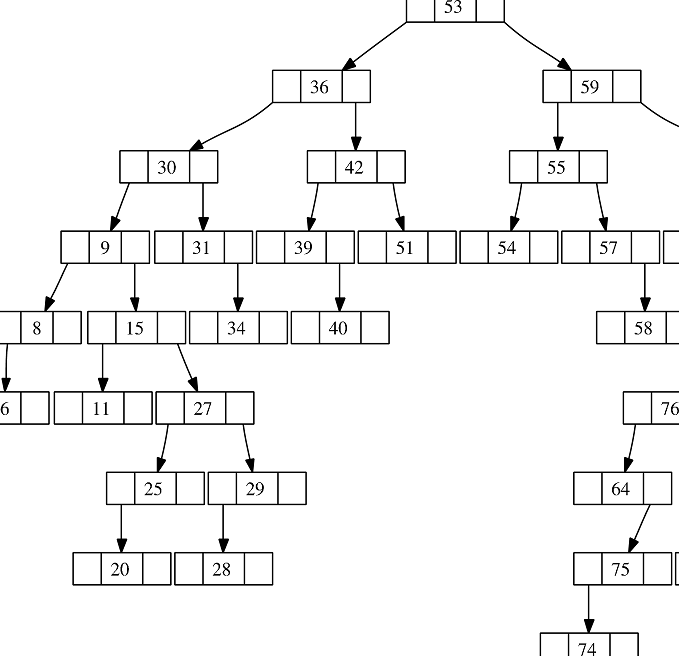
\includegraphics[width=0.8\linewidth]{images/figura_1}
   \caption{Ejemplo de figura}
   \label{chapter:intro}
\end{figure}


\begin{lstlisting}[language=json,firstnumber=1,caption={Un listado}]
{"menu": {
  "id": "file",
  "value": "File",
  "popup": {
    "menuitem": [
      {"value": "New", "onclick": "CreateNewDoc()"},
      {"value": "Open", "onclick": "OpenDoc()"},
      {"value": "Close", "onclick": "CloseDoc()"}
    ]
  }
}}
0123456789
\end{lstlisting}


%%%%%%%%%%%%%%%%%%%%%%%%%%%%%%%%%%%%%%%%%%%%%%%%%%%%%%%%%%%%%%%%%%%%%%%%%%%%%%%
\newpage{\pagestyle{empty}}
\thispagestyle{empty}

\chapter{\LARGE Título del Capítulo 2}
\label{chapter:dos}

Los capíulos intermedios servián para cubrir los siguientes aspectos: antecedentes, problemática o estado del arte, objetivos, fases y desarrollo del proyecto.

\bigskip
En el capítulo anterior se ha introducido bla, bla, bla ....

\section{Primera sección de otro capitulo}

\begin{figure}[htb]
   \centering
   
\includegraphics[width=0.5\linewidth]{images/by-nd_88x31}
   \caption{Otra figura}
   \label{chapter:intro}
\end{figure}



%%%%%%%%%%%%%%%%%%%%%%%%%%%%%%%%%%%%%%%%%%%%%%%%%%%%%%%%%%%%%%%%%%%%%%%%%%%%%%%
\newpage{\pagestyle{empty}}
\thispagestyle{empty}

\chapter{\LARGE Título del Capítulo 3}
\label{chapter:tres}

Los capítulos intermedios servirán para cubrir los siguientes aspectos: antecedentes, problemática o estado del arte, objetivos, fases y desarrollo del proyecto.

\bigskip
Bla, Bla, Bla, .....

\section{Primera sección de este capítulo}
\section{Segundo apartado de este capítulo}
\section{Tercer apartado de este capítulo}

%%%%%%%%%%%%%%%%%%%%%%%%%%%%%%%%%%%%%%%%%%%%%%%%%%%%%%%%%
\newpage{\pagestyle{empty}}
\thispagestyle{empty}

\chapter{\LARGE Título del Capítulo 4}
\label{chapter:cuatro}

Los capítulos intermedios servirán para cubrir los siguientes aspectos: antecedentes, problemática o estado del arte, objetivos, fases y desarrollo del proyecto.

\bigskip
El capítulo 1 se describió bla, bla, bla …

%%%%%%%%%%%%%%%%%%%%%%%%%%%%%%%%%%%%%%%%%%%%%%%%%%%%%%%%%
\newpage{\pagestyle{empty}}
\thispagestyle{empty}

\chapter{\LARGE Conclusiones y líneas futuras}
\label{chapter:Resultados}

Este capítulo es obligatorio. Toda memoria de Trabajo de Fin de Grado debe incluir unas conclusiones y unas líneas de trabajo futuro 

%%%%%%%%%%%%%%%%%%%%%%%%%%%%%%%%%%%%%%%%%%%%%%%%%%%%%%%%%
\newpage{\pagestyle{empty}}
\thispagestyle{empty}

\chapter{\LARGE Summary and Conclusions}
\label{chapter:Conclusiones}

This chapter is compulsory. The memory should include an extended summary and conclusions in english. 

%%%%%%%%%%%%%%%%%%%%%%%%%%%%%%%%%%%%%%%%%%%%%%%%%%%%%%%%%
\newpage{\pagestyle{empty}}
\thispagestyle{empty}

\chapter{\LARGE Presupuesto}
\label{chapter:presupuesto}

Este capítulo es obligatorio. Toda memoria de Trabajo de Fin de Grado debe incluir un presupuesto.

\section{Sección Uno}

\begin{center}
\begin{tabu} to 0.8\textwidth { | X[l] | X[l] | }
 \hline
 \multicolumn{1}{|c|}{\bf Tipos} & \multicolumn{1}{|c|}{\bf Descripción} \\
 \hline
 AAAA  & BBBB \\
 \hline
 CCCC  & DDDD \\
 \hline
 EEEE  & FFFF \\
 \hline
 GGGG  & HHHH \\
 \hline
\end{tabu}
\end{center}

\begin{table}[htb]
   \centering
   \caption{Resumen de tipos}
   \label{chapter:presupuesto}
\end{table}

%%%%%%%%%%%%%%%%%%%%%%%%%%%%%%%%%%%%%%%%%%%%%%%%%%%%%%%%%
\newpage{\pagestyle{empty}\cleardoublepage}
\thispagestyle{empty}

\begin{appendix}

\chapter{\LARGE Título del Apéndice 1}
\label{appendix:1}
\section{Algoritmo XXX}
\label{Apendice1:XXX}

\begin{lstlisting}

/**********************************************************************
*
* Fichero .h
*
***********************************************************************
*
* AUTORES
*   
*
* FECHA
*   
*
* DESCRIPCION
*   
*
***********************************************************************/

\end{lstlisting}

\section{Algoritmo YYY}
\label{Apendice1:YYY}

\begin{lstlisting}


/*********************************************************************
 *
 * Fichero .h
 *
 *********************************************************************
 *
 * AUTORES
 *
 * FECHA
 *
 * DESCRIPCION
 *
 *
 *********************************************************************/
 
\end{lstlisting}

\section{Algoritmo ZZZ}
\label{Apendice1:ZZZ}

\begin{lstlisting}


/*********************************************************************
 *
 * Fichero .h
 *
 *********************************************************************
 *
 * AUTORES
 *
 * FECHA
 *
 * DESCRIPCION
 *
 *
 *********************************************************************/
 
\end{lstlisting}



\chapter{\LARGE Título del Apéndice 2}
\label{appendix:2}
\section{Otro apéndice: Sección 1}
texto

\section{Otro apéndice: Sección 2}
texto

\end{appendix}

%%%%%%%%%%%%%%%%%%%%%%%%%%%%%%%%%%%%%%%%%%%%%%%%%%%%%%%%%%
% Aquí figurará la bibliografía

\bibliographystyle{plain}
\bibliography{memtfg}
%%%%%%%%%%%%%%%%%%%%%%%%%%%%%%%%%%%%%%%%%%%%%%%%%%%%%%%%%%

\end{document}

